\chapter{A Semantic Speech Editing Interface for Radio Production}

\section{Introduction}
Speech is a natural form of communication which is rich in information. Since
the early twentieth century, radio broadcasting has been used to transmit and
consume speech-based content. Today, radio listenership remains high and
podcasting continues to grow in popularity. 

Although many radio programmes are still broadcast live, a large proportion are
pre-recorded and put together using audio editing software. Efficient
navigation and editing of speech is crucial to the radio production process.
However, unlike text, speech must be consumed sequentially, and does not
naturally support visual search techniques \cite{Wolfe2004}. 

Audio editing interfaces display a visual representation of the amplitude of
the sound, called a `waveform'. This allows users to visually search and scan
audio content. Although the waveform is useful for many editing tasks, it
displays very limited information, especially when zoomed out
\cite{Loviscach2011}.

Semantic audio analysis technology can be used to extract higher-level
information from the sound, such as whether it is speech or music
\cite{Panagiotakis2005}, where different people are speaking
\cite{AngueraMiro2012} or a transcript of what they are saying. Presenting this
information to the user could allow them to navigate and edit audio content
much more efficiently.

In this paper, we investigate semantic speech editing in the context of
professional radio production. We explore the current production process,
including the workflow and tools that are used. We then introduce a semantic 
audio editing system that automatically transcribes speech recordings, and
allows users to navigate and edit the speech using the text of the transcript.
We evaluate this system though a qualitative study of professional radio
producers who use the semantic editor to create radio programmes for broadcast.

% RESEARCH QUESTIONS?

\section{Related work}
%For example, it can be
%used to distinguish between music and speech \cite{Wieser2014}, show where
%different people are speaking \cite{AngueraMiro2012}, and who those people are
%\cite{Doddington1985}. These technologies have successfully been combined to
%create an enhanced interface to large speech archives as part of the BBC World
%Service Radio Archive
%prototype\footnote{\url{http://worldservice.prototyping.bbc.co.uk/}}.

%Other methods of improving speech navigation have been explored, including time
%compression \cite{Arons1997} to increase playback speed, and using dichotic
%presentation \cite{Ranjan2006} to play different parts of the speech into each
%ear.
Automatic speech recognition technology makes it possible to extract partially
accurate transcripts of speech recordings. A number of researchers have
experimented with using these transcripts to enhance interfaces for interacting
with audio content.

%\subsection{Navigation}
SCAN \cite{Whittaker1999} was an interface designed to support retrieval from
speech archives. It used automatically generated transcripts to allow users to
search for keywords, and to visually search the recording by reading the
transcript. This system was developed into SCANMail \cite{Whittaker2002}, an
interface designed for interacting with voicemail. It added a number of
features including paragraph segmentation and the ability to skip to a point in
the transcript by clicking on it. The interface was later enhanced with error
correction functionality \cite{Burke2006}.

Evaluations of SCANMail found that the transcript display enabled users to
visually scan the content of the recordings to quickly extract information and
judge which bits were relevant, without having to play the audio.

%\subsection{Editing}
Transcripts have also been used to enhance interfaces for editing audio.
Whittaker and Amento \cite{Whittaker2004} created an interface that allowed
users to select part of a transcript, then cut and paste that selection.
This operation also edited the underlying audio to match the text.
Their formal evaluation found that this `semantic editing' was faster and as
accurate as editing with a waveform-based interface, even when the accuracy of
the transcription was poor.

More recently, Rubin et. al. \cite{Rubin2013} presented a novel interface for
creating `audio stories' that combine speech and music. The interface displayed
a transcript with two columns to distinguish between speakers. It allowed the
user to cut, copy, paste and delete the audio using the transcript text.  It
also annotated the transcript to indicate repeated phrases, `umm's, breaths and
pauses. To enable this functionality, the system relied on manual transcription
and annotation which provided accurate results but was very expensive. In an
informal evaluation, the editing capabilities received positive feedback.

%\subsection{Time compression}
A number of studies \cite{Whittaker2002,Vemuri2004,Ranjan2006} have also
combined transcript displays with time-compression to speed up playback of
audio.  They found that having a transcript improves comprehension and allows
faster playback.

%Dichotic presentation, in which different parts of a recording are played into
%each ear, was also tested \cite{Ranjan2006}.

%\begin{figure}
%\centering
  %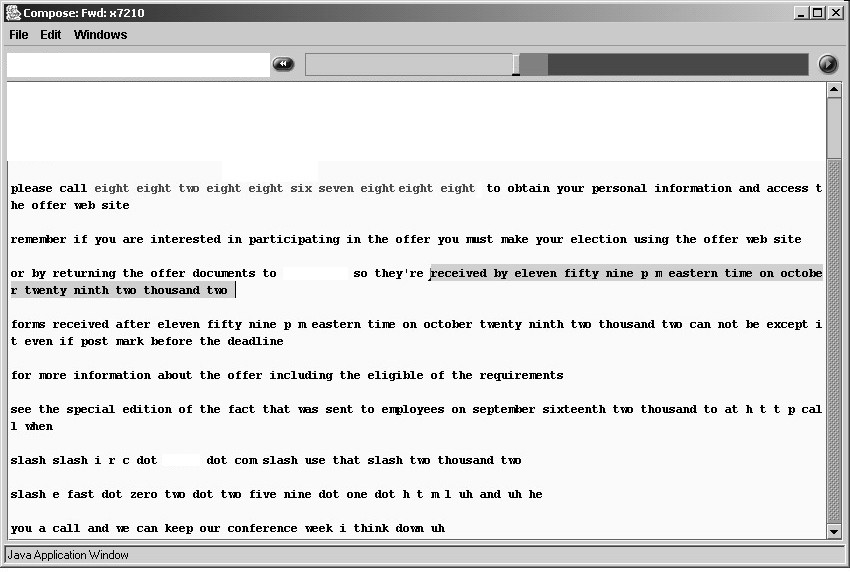
\includegraphics[width=\columnwidth]{figs/whittaker2004.png}
  %\caption{Semantic speech editor \cite{Whittaker2004}}
  %\label{fig:semanticeditor}
%\end{figure}

%, which has been shown to improve the speech and
%accuracy of audio search \cite{Ranjan2006,Whittaker2000} and comprehension
%\cite{Vemuri2004}. Word-level timing information, also allow users to edit
%speech using a text-based interface \cite{Whittaker2002,Burke2006,Rubin2013}.
%Even with imperfect transcriptions, editing using this technique is faster and
%as accurate as acoustic editing \cite{Whittaker2004}.

%Later systems have improved these interfaces with editing \cite{Burke2006},
%confidence shading \cite{Burke2006} and highlighting breaths, pauses and
%repetition \cite{Rubin2013}.

These studies have demonstrated the potential that transcript-based interfaces
have for improving the navigation and editing of audio content. However, they
have not yet been tested under real-world conditions.

In this paper, we present a semantic speech editing system that was evaluated
in a professional radio production environment. Gaining access to these
environments can be difficult. A number of studies on television production
systems have been conducted \cite{Engstroem2010,Perry2009}, but we were unable
to find any on radio production. One study attempted to recruit radio producers
but was unsuccessful \cite{Kim2003}.

\section{Pilot study}
A short previous study of radio production at the BBC investigated how semantic
audio technology could best be applied in the context of radio production.  The
results are fully documented in \cite{Baume2015}, but a short summary is given
below.

%In order to determine how these technologies would be best applied in the
%context of radio production, we conducted a short pilot study of radio
%production at the BBC, the results of which are more fully documented in
%\cite{Baume2015}.

%, which explored the workflow, roles, motivations and
%environmental factors.

The objectives of the study were to discover how radio programmes are created,
and to identify any opportunities to improve the process using technology.
Three representative but varied programmes were studied -- a news bulletin, a
drama and a documentary. The producers of each programme were observed and
interviewed to fully document their workflow, which took between half a day
(for news) and four days (for the documentary).

The study found that radio producers rely strongly on scripts and transcripts of
speech recordings. For example, after the observed documentary makers recorded
an interview, they `logged' each one by listening through and writing notes, or
using a third-party to write a full transcript for them. Both methods cost
time and money. The programme is then edited using just the notes or transcript
(known as a `paper edit'). During this period there was no easy way to listen
to the audio, so although they know \textit{what} was said, they don't know
\textit{how} it was said.

After editing on paper, the producer had to go back to find and cut each
piece of audio they wanted to use in the programme, known as a `rough edit'.
Converting from audio to text and back again is costly, but is considered by
the producers to be worthwhile.
We believe that by linking audio and text representations together in an
editing system, it would be possible to work with either representation without
incurring the cost of converting between the two.

 %It found that producers of speech radio prefer to work with
%text-based representations of audio rather than with the recordings directly.
%Their workflows are primarily paper-based which creates extra work when moving
%between paper and audio. Creating a link between the words on the paper and
%their location in the audio recordings could significantly improve the
%production workflow.

%The study also identified opportunities to apply semantic audio technology
%and interaction design to radio production tasks. Lots of time is spent
%cleaning up recordings by removing redundant speech, which could be fully or
%semi-automated. Segmenting speech content by speaker would make a positive
%impact on most speech-based tasks. Finally, drama productions could benefit
%from an easy way to compare multiple takes of the same scenes.

\begin{figure*}
\centering
  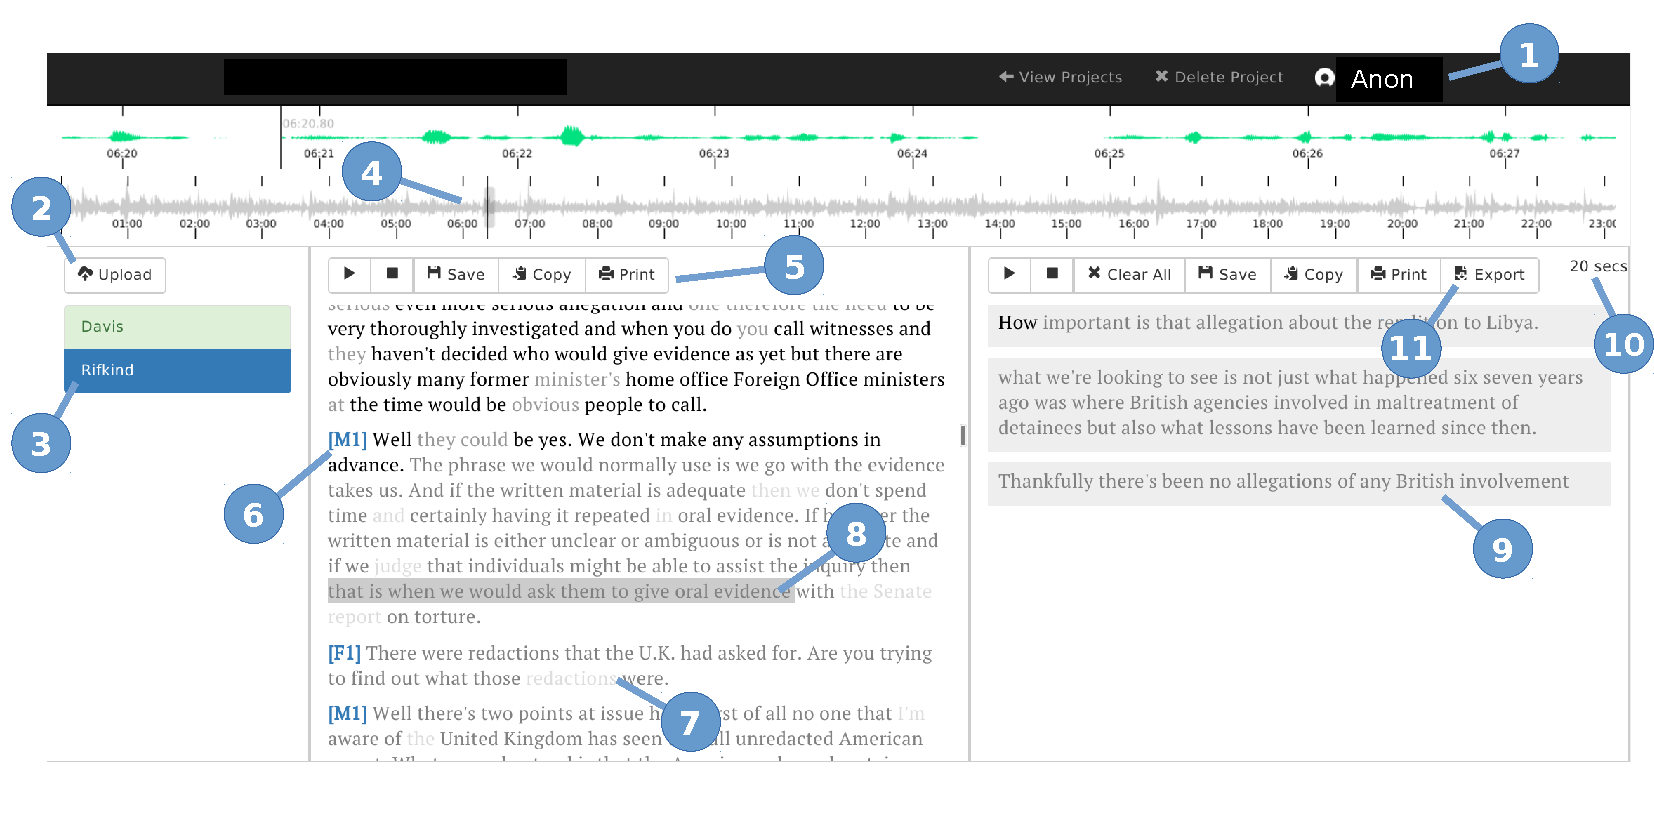
\includegraphics[width=\columnwidth]{figs/interface-labels.pdf}
  \caption{Screenshot of the user interface with highlighted features: (1)
    individual user accounts and projects, (2) upload of audio recordings, (3)
    list of uploaded recordings, (4) waveform display of currently selected
    recording, (5) toolbar with playback, save, copy and print functionality,
    (6) transcript of selected recording with speaker labelling and word
    editing, (7) confidence shading, (8) transcript selection with
    drag-and-drop editing, (9) listing and re-ordering of edits, (10) duration
    of edit, (11) export edit to audio file or digital audio workstation.}
  \label{fig:interface}
\end{figure*}

\section{Semantic speech editing system}
A browser-based semantic editing system was created to assist with logging and
rough editing of speech recordings. It allows users to upload audio recordings
which are automatically transcribed and presented in a text-based interface
that allows them to navigate and edit the audio using the transcript.
This system differs from those used in previous research by including the
ability to export professional quality audio in a number of formats, which
enables it to be used for radio production.

%This section describes the design, features and implementation of the
%prototype.

\subsection{Design}
The system was designed to offer basic functionality for creating a rough edit,
and to easily fit into the existing production workflow. A screenshot of the
interface and numbered list of the main features are shown in
Figure~\ref{fig:interface}.

\subsubsection{Layout}
The interface is laid out so that the workflow operates from left to right.
Recordings are uploaded and listed on the left (2), the transcript of the
currently selected recording is shown in the middle (6), and the clips are
created and exported on the right (9). The waveform of the currently selected
recording is shown at the top on a dual time-line (4), where the bottom
waveform shows the entire recording and the top is a magnified display of the
current position.

\subsubsection{Navigation}
Users can navigate the selected recording by clicking on a word in the
transcript, which seeks to that position and starts playback, or by clicking on
the waveform to jump to a specific time. Playback can also be controlled using
buttons in the toolbar above the transcript (5).

The text before and after the current playback position is coloured black and
dark grey, respectively, to indicate the current playback position in the
transcript.  Words which the speech recognition system is not confident about
are shaded in light grey (7), known as `confidence shading'.

Following early informal feedback, features were added to allow the text to be
corrected, printed and copied into a word processor. If a word is
incorrect, it can be fixed by double-clicking it, typing the new word and
pressing enter. The text of the transcript or clips can be copied or printed by
clicking the copy or print buttons (5).

\subsubsection{Editing}
An audio clip can be created from the transcript using drag-and-drop.  The user
selects text from the transcript (8) then drags and drops the selection in the
space to the right.  Each clip is contained in a shaded box (9) which can be
re-ordered by dragging them up and down, or deleted by clicking an `X' in the
top right of the box.

The clips can be played using the playback buttons at the top, or by clicking
on a word. The total length of the clips is displayed above the text (10).  The
clips can be exported as a single .wav audio file or an `edit decision list'
(EDL) using the export button (11). An EDL contains metadata about which parts
of the recording make up an edit.

\subsection{Implementation}
The system was implemented using web standards, which allowed a consistent
experience on any recent web browser, and avoided the need to install any
software locally. The front-end was written in Javascript using the Hyperaudio
\cite{Hyperaudio} and peaks.js \cite{Peaks} libraries, and the back-end was
built using Node.js and MongoDB running on a virtualised Ubuntu server.
Communication between the two was done through a REST API.

\subsubsection{Transcription}
Uploaded recordings were automatically transcribed using a state-of-the-art
commercial automatic speech recognition web
service (\url{https://www.speechmatics.com/}).
In an informal evaluation of the system which used 48 hours of mixed genre
television content, it had an overall word error rate of 47\%.  For
news content, which is clearly spoken by a native speaker, this dropped to
16\%. As speech on radio is similar in nature to speech on television news, the
error rate was comparable. However recordings with non-native speakers had a
higher error rate.

The speech-to-text system can recognise esoteric words like `ribosome' and
`ARPANET', but can struggle with colloquialisms and casual conversation. If the
recording is too quiet or noisy, or a word isn't in its dictionary, the system
makes a best guess (e.g.  `subbuteo' was translated as `some beauty'). It also
attempts to detect where there is a change of speaker, and to give each speaker
a unique label including their gender (e.g. M2, F5). These are marked in the
interface with a new paragraph and square brackets containing the speaker ID.

The time taken by the transcription service to process each uploaded recording
was approximately half as long as the length of the recording.  The time
depends primarily on the length of the recording but also on noise, accents and
the complexity of the speech.

%\begin{figure}
%\centering
  %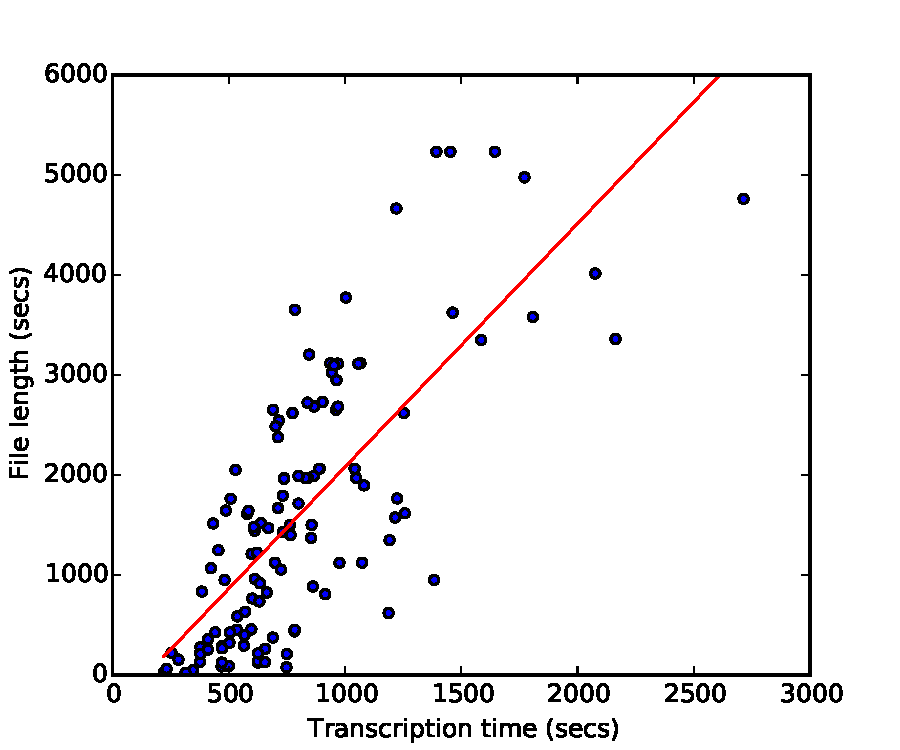
\includegraphics[width=\columnwidth]{figs/transcribetime.pdf}
  %\caption{Time taken to transcribe each recording with linear trend line}
  %\label{fig:transcribetime}
%\end{figure}

\subsubsection{Export}
Three options to export edited audio were implemented. The first option
exported a single .wav audio file of the edit by using the program Sox. The
other two options exported EDLs for the most common audio editors used at the
BBC -- SADiE, made by Prism Sound, and dira! StarTrack, made by SCISYS. These
were written using Python scripts.

The .wav export method is a `destructive' edit, in that it throws away the
pieces of the recording which weren't selected. The EDL exports are
`non-destructive' edits because the full original recordings are retained and
the edit points can be re-adjusted.

\subsection{System features}
This section lists and describes the features of the prototype system developed
for the evaluation.

\subsubsection{User accounts}
Access to the system is managed through user accounts. Accounts can only be
created by the experimenter. User authentication is handled using the BBC iD
sign-in system\footnote{\url{http://www.bbc.co.uk/id/info}}.

\subsubsection{Projects}
Each user can create multiple projects in order to keep their work organised.

\subsubsection{Upload}
Users can upload their own audio recordings to the system.  Each recording can
be given a name to identify it. When uploading a recording, the user is
prompted to specify whether the accent of the speaker is British or American
(to assist the automatic speech recognition), and agree to a disclaimer about
the security of uploading content.

After upload, the recordings are converted to 16-bit 48kHz stereo WAV format,
an MP3 `scratch' version is created and the scratch version is sent to a
third-party speech-to-text service.

\subsubsection{Transcript alignment}
As part of the upload feature, the user can optionally upload a transcription
of the recording in .docx format. The text from the uploaded transcript is
considered to be a perfect verbatim transcription. The text is aligned to the
output of the speech-to-text system so that a timestamp is then attached to
each word of the uploaded transcript.

\subsubsection{Transcript display}
The transcript of the uploaded recording (either automatic or aligned) is
displayed to the user in the system interface. When the user clicks on a word,
the recording starts playing back from the time that word is spoken.

\subsubsection{Transcript editing}
The user can edit the recording's transcript by double-clicking on a word,
typing the new word and pressing \texttt{Enter}. Their changes can be saved by
pressing a Save button at the top of the transcript display.

\subsubsection{Waveform display}
An audio waveform is displayed at the top of the interface. The waveform
display is split into two rows. The bottom row displays the waveform from the
entire recording, from beginning to end. The top row displays a `zoomed-in'
subset of the bottom row, dependent on the current position of the playback.

\subsubsection{Clipping}
Users can create an audio clip by highlighting text in the transcript column on
the left, then dragging the highlighted text into the edit column on the right.
Clips from different recordings can be combined into a single edit.  The clips
in the edit column can be played, paused and stopped by the user.

\subsubsection{Clip re-ordering}
Clips in the edit column can be re-ordered by dragging them up or down. As
a clip is being dragged, the other clips move dynamically to make space for it.

\subsubsection{Copy}
The transcript and edit columns each have a `copy' button. This opens a dialog
with a text box of the transcript or edit text, with the text automatically
selected. The dialog explains to the user that they can copy the text by
pressing \texttt{Ctrl + C}.

\subsubsection{Print}
The transcript and edit columns each have a `print' button. This launches the
browser's print feature with the text of the transcript or edit. The user can
then continue the normal process of printing a document.

\subsubsection{Export}
The audio of the edit created by the user can be exported in a number of
different formats. The first is the uncompressed audio format WAV. This cuts
together the desired clips using the original recordings and concatenates them
into one recording. As the original recordings are used, the sound quality is
identical. However, the unselected bits of the recording are not exported,
meaning that the user can't easily readjust the edit points after exporting.

The other two formats are compatible with the BBC's two most popular DAWs --
SADiE and dira! Startrack. In each of these cases, the exported file includes
the full original recordings of each clip used, and an `edit decision list'
(EDL), which describes the in and out points of each edit. This means that the
user can use the DAW's interface to easily readjust edit points and add other
content such as music, presenter links and sound effects.

\subsection{System implementation}
The prototype system was created using modern web technologies. This approach
means that it can be accessed using the internet and is compatible with any
modern web browser on any computer platform. The abundance of well-supported
software libraries for these technologies also mean that development can be
done very quickly.

\subsubsection{Back-end}
The back-end of the system runs on a virtualised Ubuntu 14.04 server at BBC
R\&D. The NodeJS platform is used with the Express framework to run the web
services. MongoDB is used as a database for storing user information and the
metadata of recordings, projects and edits. Uploaded audio is processed using
FFmpeg, then sent to a third-party speech-to-text service using a REST API. The
logging library Bunyan is used to keep a detailed track of user and system
events.

\subsubsection{API}\label{sec:api}

\begin{table}[ht]
\begin{tabular}{ l l l l }
Method & Type & Address & Description \\
\hline
\texttt{GET}    & \texttt{HTML} & \texttt{/} & Show front page \\ 
\texttt{GET}    & \texttt{HTML} & \texttt{/projects} & Show user's projects \\ 
\texttt{GET}    & \texttt{HTML} & \texttt{/projects/\{projectId\}} & Show
interface for project \\
\texttt{POST}   & \texttt{JSON} & \texttt{/projects} & Create new project \\
\texttt{GET}    & \texttt{JSON} & \texttt{/listProjects} & List existing
projects \\
\texttt{GET}    & \texttt{JSON} & \texttt{/listAssets/\{projectId\}} & List
assets of project \\
\texttt{PUT}    & \texttt{JSON} & \texttt{/projects/\{projectId\}} & Update
project \\
\texttt{DELETE} & n/a           & \texttt{/projects/\{projectId\}} & Delete
project \\
\texttt{GET}    & \texttt{HTML} & \texttt{/projects/\{projectId\}/mix} & Get
edit for project \\
\texttt{POST}   & \texttt{JSON} & \texttt{/projects/\{projectId\}/export} &
Export edit using given format \\
\texttt{POST}   & \texttt{Form} &\texttt{/upload} & Create new asset \\
\texttt{GET}    & n/a           & \texttt{/assets/\{type\}/\{assetId\}} &
Download data of given asset \\
\texttt{PUT}    & \texttt{JSON} & \texttt{/assets/\{assetId\}} & Update asset \\
\texttt{DELETE} & n/a           & \texttt{/assets/\{assetId\}} & Delete asset \\
\texttt{POST}   & \texttt{Form} & \texttt{/token} & Create token for new user
\textit{(admin only)} \\
\texttt{GET}    & \texttt{HTML} & \texttt{/signup?token=} & Create new user
using token \\
\texttt{POST}   & \texttt{JSON} & \texttt{/log} & Post message to system log \\
\end{tabular}
\caption{Description of the system API}
\end{table}

\section{Study design}
The goal of our study was to explore how radio programmes are currently
created, and to evaluate the semantic editing system in a professional radio
production environment.  The within-subjects study was primarily qualitative
and was conducted through observation and interviews. Some basic metrics such
as task completion time were also recorded.

\subsection{Participants}
The study used professional radio producers with at least five years of
experience. To make the most of the available access, we recruited participants
exclusively from the BBC Radio division. Participants were invited via email
that was sent to a variety of departments in radio.

Drama programmes were excluded from the study as their production workflow
involves making multiple recordings of lines in a script and selecting the best
ones \cite{Baume2015}. This is a sufficiently different process to other
programme genres that it warrants a different interface.

Five participants (P1--P5) were recruited (4 male, 1 female) who each had
between 6 and 20 years experience in working as a radio producer. Due to the
length and complexity of the study, this was the maximum number that could take
part in the time available, but this should be sufficient to identify most
usability problems \cite{Nielsen1993}.

The participants produced programmes of different lengths from a range of
genres: P1 produced a single 27-min documentary, %plus 50-min for WS
P2 produced a 27-min documentary as part of a ten-part series, P3 produced a
single 45-min documentary, P4 produced a 14-min archive programme (based around
material from the archive) as part of a ten-part series, and P5 produced a
single 27-min magazine show (covering multiple stories on a single theme).

\subsection{Procedure}
Radio producers are very busy and find it difficult to step away from their
work for too long. To account for this, the study was designed to take place at
their desk and overlap as much as possible with the work they need to do.
The design was made up of the following five stages:
\begin{enumerate}
  \item A semi-structured interview to learn about the participant's
    background, their existing production workflow and the tools they used as
    part of that. The interviews took between 30 and 40 minutes.

  \item A short training session on the semantic editor interface, followed by
    a usability test.  Each participant was trained on the interface's
    functionality using a pre-written `tool-tip tour', in which the participant
    was presented with a sequence of instructional pop-up dialog boxes overlaid
    on the interface.  This ensured consistency of training between
    participants.

    The usability test involved giving the participant a series of verbal
    instructions for common tasks that utilised all of the functionality of the
    interface. The investigator observed their actions, but gave no other
    directions unless requested. They noted any unexpected behaviour, stumbling
    blocks or other failures.

  \item An observation of the participant as they produce a radio programme.
    The task that was observed was logging and rough editing a recording for a
    programme they were working on.  The task was observing twice -- once using
    the existing workflow and once using the semantic editing system.  Similar but
    different audio content was used for each task so that the participant
    wasn't already familiar with the material (e.g. editing two interviews).
    The order of the conditions was counterbalanced to eliminate bias.  The
    actions of the participant on the semantic editing system were logged
    electronically, and after the observation they were asked to rate each
    condition using the NASA Task Load Index metrics \cite{Hart1988}.

    The tasks were performed as part of the production of a radio programme,
    and the observation was done in the participant's normal work environment.
    The investigator sat beside the participant during the task and made notes
    on the workflow, tools, generated metadata, usability issues, task
    completion time, and unexpected reactions or usage.

  \item A semi-structured interview about the participant's experience of each
    system and how they compare. The primary objective of this interview was to
    extract the advantages and disadvantages of each workflow. The interviews
    took between 30 and 60 minutes. The audio from each interview was recorded
    and transcribed to allow a full analysis.
    %The questions asked were:

    %\begin{itemize}
        %\setlength\itemsep{0em}
      %\item Which aspects of the existing system did you / did you not find useful?
      %\item Which aspects of the prototype system did you / did you not find useful?
      %\item Overall, which system did you prefer and why?
      %%\item Did the prototype change the way you made the programme? If so, how?
    %\end{itemize}

  \item Each participant was then given access to the semantic editing system
    for a further month, and was invited to continue to use it should they
    wish. Each week, they were asked via email whether they had been using the
    system, and if so, which features they valued most/least or were missing.
    During this time, their usage of the system was also logged electronically.
\end{enumerate}

\subsection{Analysis}
The notes from the pre-interview, usability test and observation were analysed
to look for common issues, unexpected reactions and unanticipated usage. The
post-interviews were transcribed and coded using the software package RQDA
\cite{RQDA} to identify common themes. The electronic usage logs from the
semantic editor interface were analysed using custom Python scripts to
calculate and graph usage patterns.

\section{Study results}

%\subsection{Observation}
%During the first interview, participants worked with the investigator to
%identify a particular task in their workflow that would form the basis of the
%observation. In every case, logging and rough editing of an interview was
%selected, as this process takes a long time, is considered tedious and would
%benefit from automatic transcription.

%Due to the pressured and changing work environment, the observation had to fit
%around the editing requirements at the time of observation. This meant that P4
%and P5 did not do any logging during observation.

\subsection{Existing workflow}
This section describes the existing radio production workflow. The process is
documented as described by participants in the first interviews (stage 1) and as
witnessed by the investigator during the observation (stage 3).

\subsubsection{Commissioning}
Programmes begin their life when they are `commissioned'. Producers pitch ideas
to a commissioning editor who selects which ideas and producers to fund. Some
programmes are commissioned for a series or a regular ongoing slot. These tend
to be topical and have a short turn-around period. The subject matter is chosen
by the producer between a week and a month before transmission. Other
programmes are one-off productions which have a longer turn-around time. These
tend to cover bigger subjects in greater depth.

\subsubsection{Research}
After the topic has been chosen, the producer researches the subject in greater
detail. This is done by reading, listening and watching existing material on
the subject, and finding and talking to relevant people. The objectives of the
research stage are to identify a compelling storyline for the programme and
find contributors to interview. During this period, the producer will also
recruit a presenter for the programme.

\subsubsection{Recording}
The producer will then arrange interviews with contributors. Often a
`pre-interview' is conducted over the phone to see what they will say and how
well they come across. The presenter and producer will then meet the contributor
in the studio, or a location relevant to the topic, to record the interview. If
the contributors are too far away, interviews can be done using a digital
`ISDN' telecommunication link to a local radio studio or using Skype.

\subsubsection{Logging}
Once material has been recorded, the producer must select which bits to use in
the programme.  This selection process is aided by creating `logs' of the
interviews. The exact format of the logs varies between individuals, but they
usually contain a very rough transcript of the interview with occasional
timestamps and notes.  The log allows the producer to quickly find and share
what was said, when and by whom.

Logs are usually written by the producer themselves. As they have done the
research and are normally present at the recordings, they can use their memory
to navigate the material and use their experience to quickly determine which
parts are relevant. Some programmes that are under particular time pressure
will use a third-party to create a verbatim transcript of a few interviews
\cite{Baume2015}, but most do not because it is very expensive.

\begin{figure}
\centering
  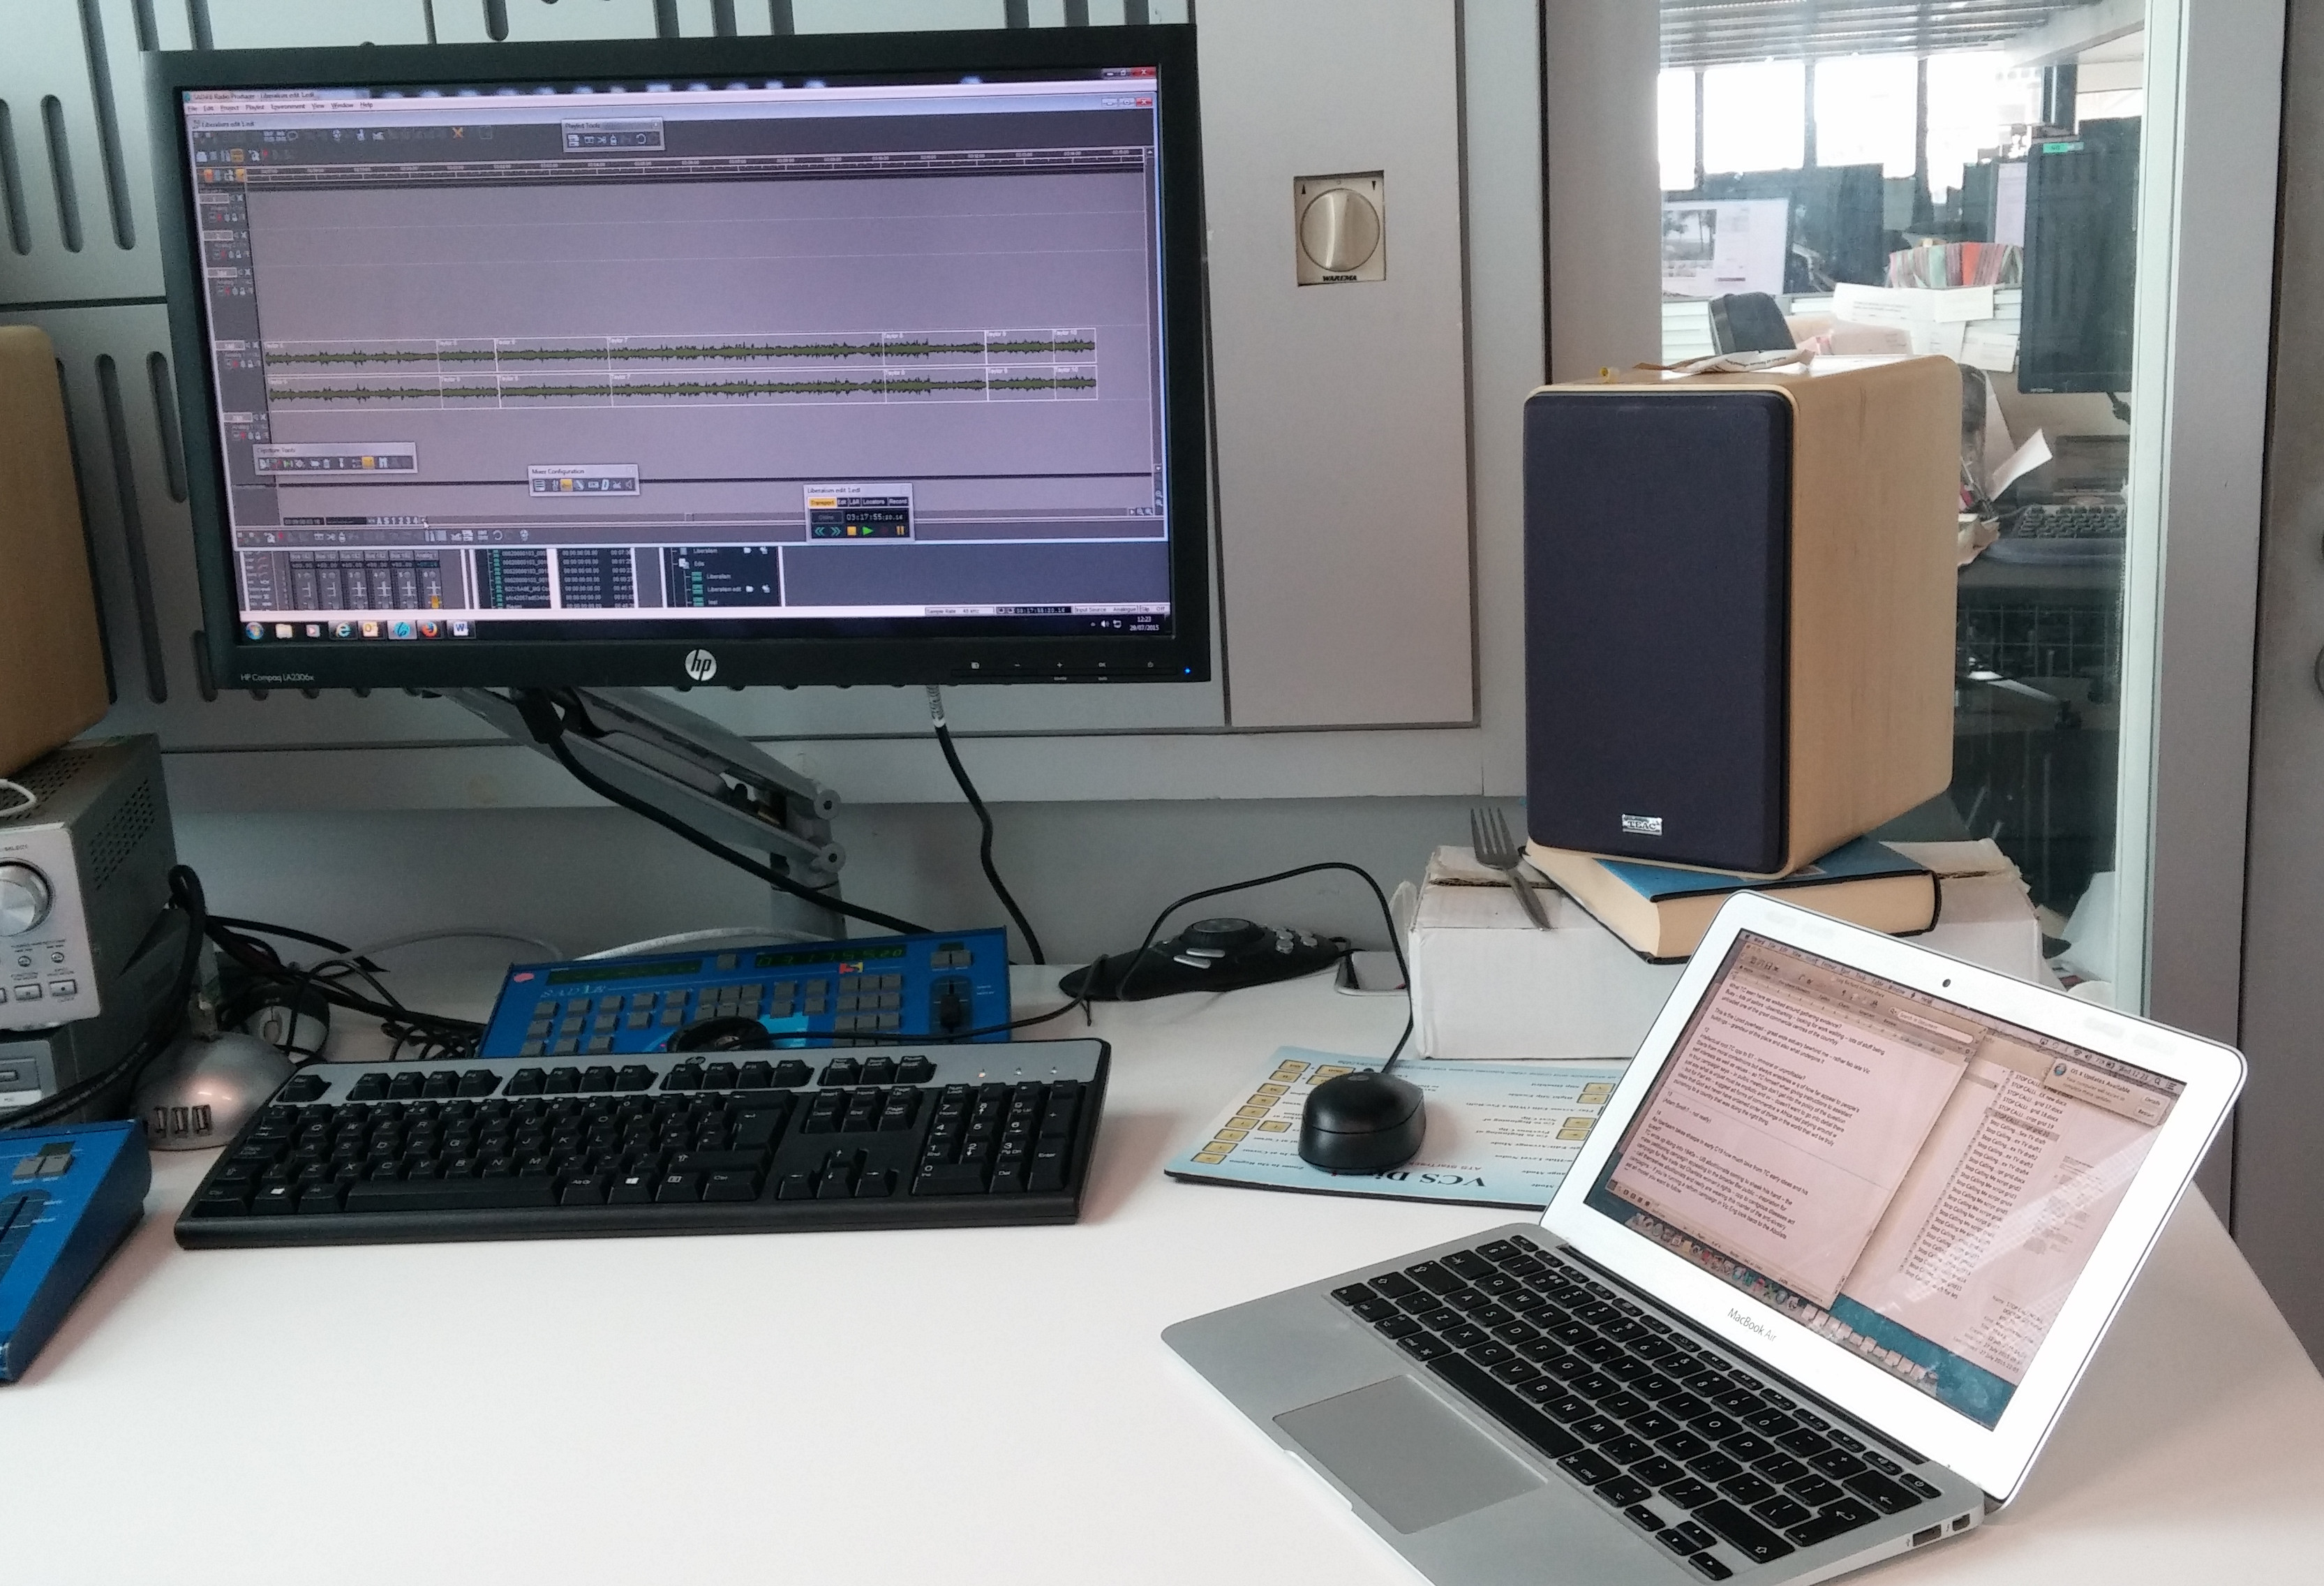
\includegraphics[width=0.5\columnwidth]{figs/phil-desk.jpg}
  \caption{P3 logging interviews with a digital audio workstation on the desktop
    PC and word processor on the laptop}
  \label{fig:desk}
\end{figure}

In the observation, P1 and P3 wrote their logs in Microsoft Word whilst using a
digital audio workstation (DAW) to play the recording (see
Figure~\ref{fig:desk}). P5 usually follows a similar process, but did not do
any logging during observation.

P4 also did not do any logging during observation, but explained that they
would normally write their logs by hand in a notebook whilst listening on a
portable music player somewhere away from the desk, such as a caf\'e.

P2 used a different approach. They played the recording in a DAW and used a
keyboard shortcut to create timed markers at any points of interest. By seeing
where the markers clustered, they identified where to make clips, then gave
each of the clips labels. This approach allowed them to focus more on the
audio, but didn't allow them to make any detailed notes.

Every participant that was observed logging played the audio faster than real
time at least once. This allowed them to fast-forward through parts of the
interview that may not be of interest (e.g. discussion in the background)
whilst still being able to listen out for anything they might want to use.

\subsubsection{Rough editing}
This stage involves extracting audio clips from the recordings which will form
the basis of a draft edit of the programme. If the recording is short and has
been done recently, as was the case for P4 and P5, this can be done without a
log. In this situation, the producer listens through the recording using a DAW
and presses a keyboard shortcut to split the recording, usually at the
beginning/end of questions/answers. They then go back and remove unwanted
segments.

If the recording has been logged, the producer will use this to decide which
bits to clip. They will use the timestamps written in the log to narrow down
their search area for each clip they extract.

At the end of this stage, the producer will have clips of their recordings
assembled into a basic structure of their programme in the DAW. This will
normally be about twice as long as the final programme, sometimes significantly
longer (e.g. P5 rough edited 22 hours for a 37-min programme). The producer
then will continue to trim the edit down to a manageable length.

\subsubsection{Links}
The next stage is to add narrative elements, known as `links' to join the clips
together into a storyline. The producer and presenter will write the links
together, using a script of the programme to collaborate. The presenter records
the links in a studio and the producer then assembles them into the edit.

\subsubsection{Fine editing}
Once all of the content has been added to the edit, the final stage is to get
it down to time, adjust the levels, and to add any music or sound effects. The
speech is cleaned up by removing redundant noises (e.g.  `umm', `err', `you
know') in a process known as `de-umming'. Many producers will bring in an
experienced sound engineer to help with any final complicated editing.
Once the editing is complete, a final version is mixed down and sent to the
producer's editor who signs it off.

\subsection{Existing tools}

\subsubsection{Digital audio workstation}
In the study, three of the participants (P3, P4 and P5) used SADiE as their
DAW. SADiE is provided to the producers by the BBC and comes with support in
the event that anything goes wrong. However, the other two participants chose
to use other software packages that aren't formally supported.

P1 used Adobe Audition because they were familiar with the interface and it was
installed on their laptop, which gave them the freedom to work anywhere.

P2 comes from a television production background and used Apple's Final Cut
Pro, which is primarily a video editor but also includes audio editing
functionality.  Similarly, P2 liked the familiar interface and having it on
their laptop. In addition, they enjoyed being able to import audio directly
from video content without having to use another program to extract the audio
first, and being able to add `titles' to their edit to make written notes.

\subsubsection{Script}
All of the participants created and maintained a `script' document of their
programme.  It was primarily used to help the producer structure their
thoughts, but was is also used to help communication with the presenter over
email. The scripts contained a varying amount of detail, depending on the
producer. Some included a full transcription of the edit, whilst others
contained a bullet-point outline. The scripts were all written using Word, with
P2 also using `MindManager' mind mapping software.

P1, P2 and P5 started their scripts during the research stage by writing an
ordered list of bullet points of topics to cover and a list of draft questions
to ask contributors. P3 and P4 waited until after they had done some interviews
to start the script, as they wanted to structure the programme around the
discussion.
P3 and P5 updated the script after every edit to ensure they were always in
sync. This added significant overhead but gave them a visual structure to
follow when making the final changes.

\subsection{Usability study}
Participants were first introduced to the semantic editing interface through a
usability study (stage 2). P1 completed the study quickly and without issue,
expressing that it was easy and intuitive. The other four participants
successfully completed the study, but identified a number of usability problems
which are outlined below.

\subsubsection{Text manipulation}
The interface was designed to allow users to copy the text of the entire
transcript by pressing a `copy' button. Four of the five participants
intuitively selected the text before pressing the copy button.  P2 expressed a
preference to use Ctrl+C and Ctrl+V shortcuts to copy and paste text, rather
than a drag-and-drop gesture.  Additionally, P2 said they wanted to be able to
remove selected text by pressing backspace, or to export only selected text.
%Future versions should
%consider allowing users to apply actions only to selected text.


Three of the five participants (P2, P3 and P5) couldn't remember the action to
correct a word (double-click). Two of them (P2 and P3) right-clicked the text
and looked for an option in the context menu.

\subsubsection{Keyboard shortcuts}
Two of the five participants (P2 and P3) instinctively pressed the space bar to
start and pause audio playback. This is a universal keyboard shortcut in all
DAWs and is ingrained in most producers, however no keyboard shortcuts were
implemented in the semantic editing system.

\subsubsection{Search}
When asked to select a certain phrase, P1, P2 and P4 instinctively pressed
Ctrl+F to search for a word in the phrase. As this feature is built into the
browser, it wasn't included in the training or study, but was discovered
anyway. The participants that used it remarked that it made finding particular
bits much easier.

%P2 confused about double waveform

%\section{New workflow}
%Following the usability study, participants were observed using the prototype
%interface to complete a common production task and interviewed about it
%afterwards. This section documents the findings.

\begin{figure}[t]
\centering
  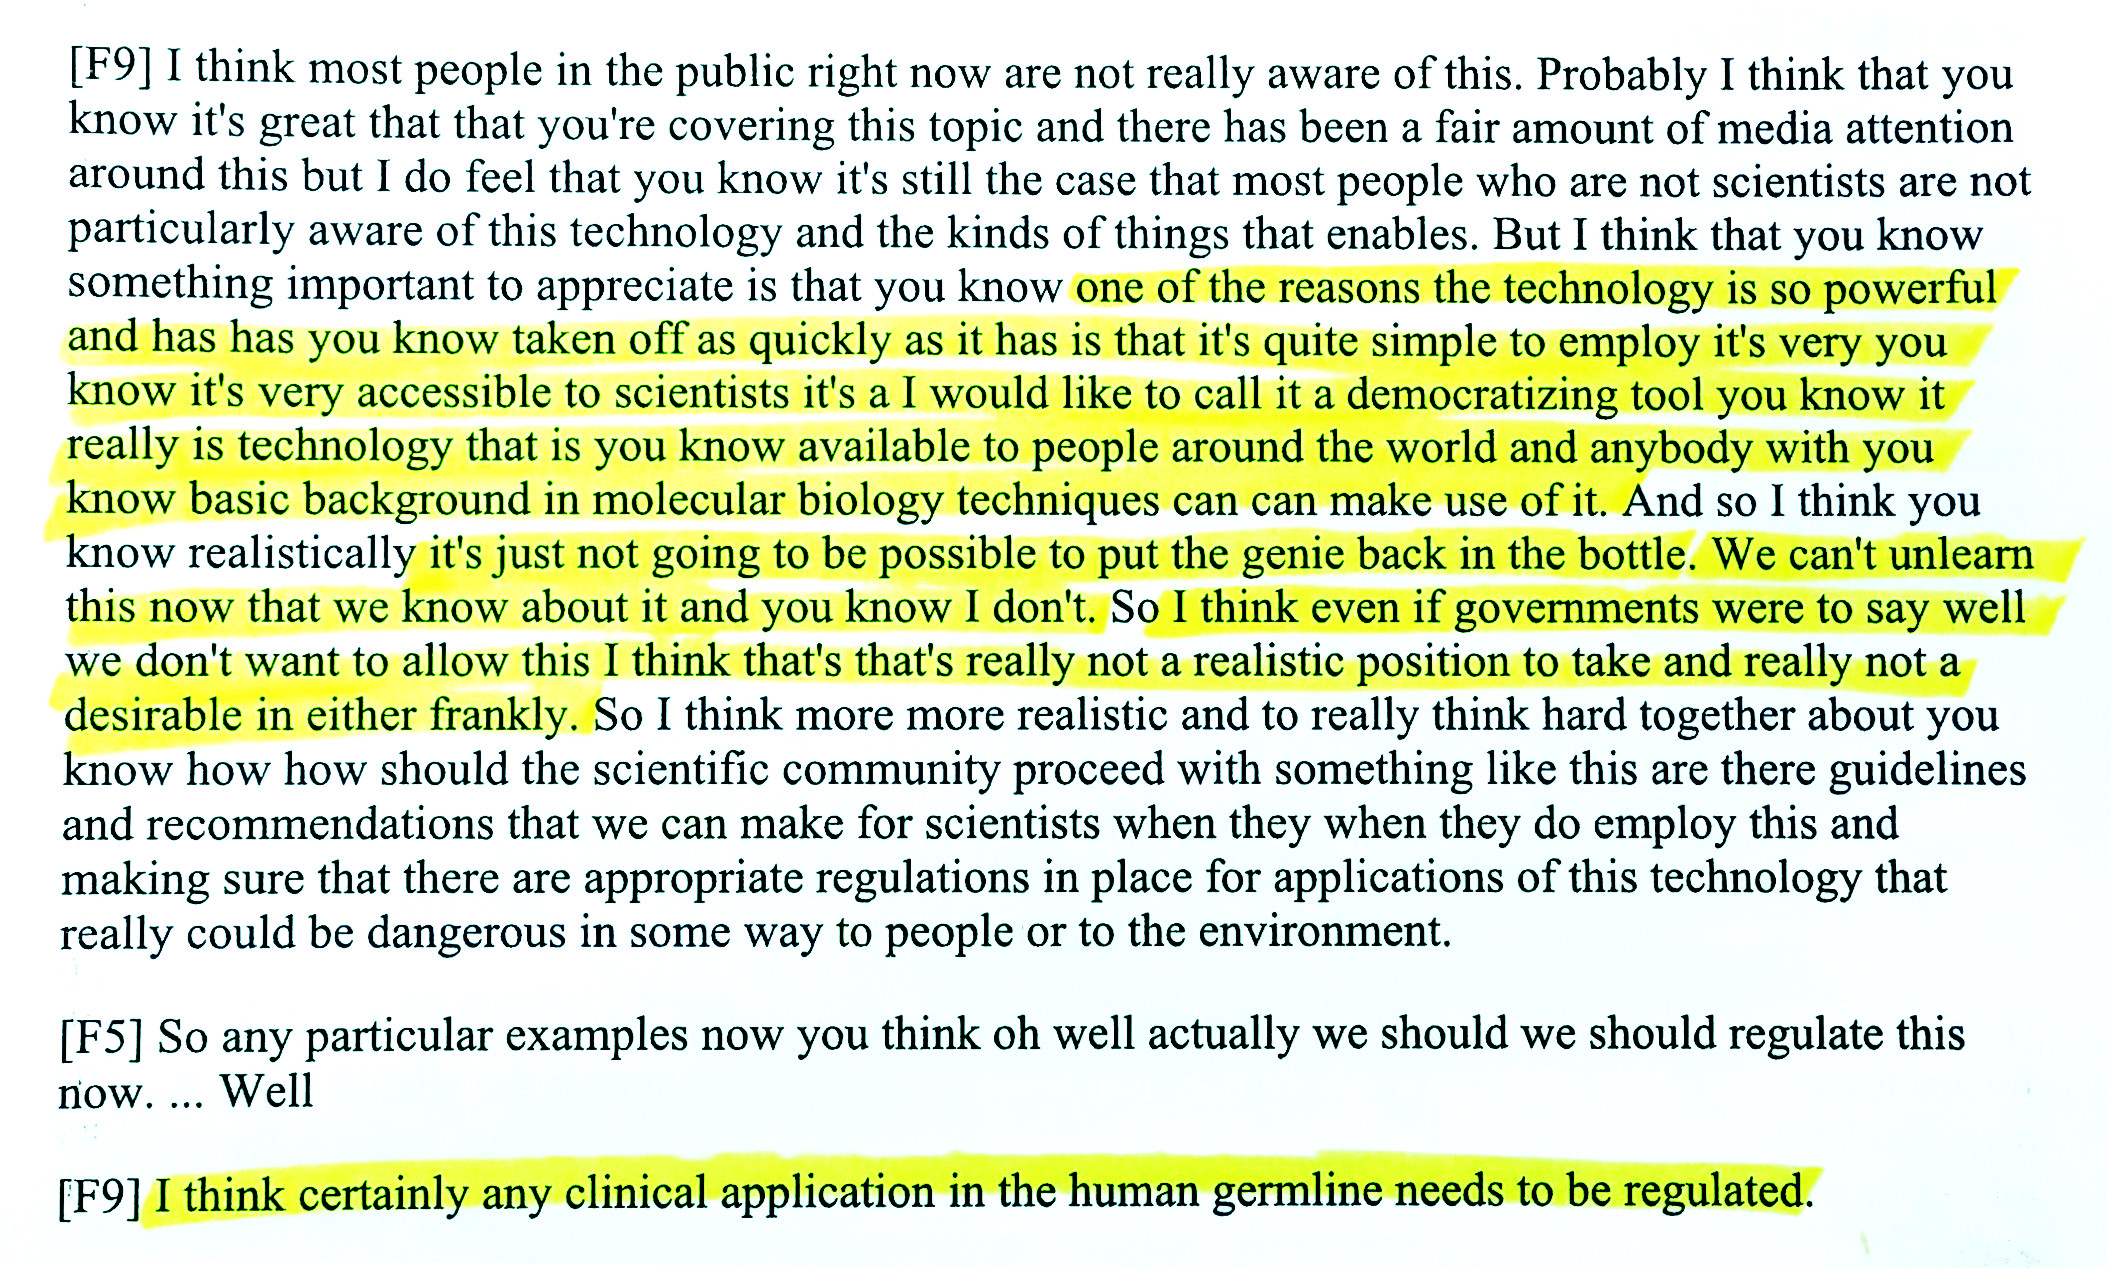
\includegraphics[width=\columnwidth]{figs/highlighting-cropped.jpg}
  \caption{P2 using a highlighter pen with a printout}
  \label{fig:highlight}
\end{figure}

\subsection{New workflow}
To evaluate the semantic editing interface, participants were observed while
they used the system to log and rough edit recordings for a programme.
Although it was designed as an all-in-one solution for putting together a rough
edit for a programme, participants used the interface in different ways to
integrate with their existing workflow.

P3, P4 and P5 used the interface much as designed by using the transcript
window to read and identify suitable clips, then dragging them across to the
edit window and exporting the audio. Each differed in how they exported the
content.

P5 made a list of all the clips they wanted for the programme before exporting
them into SADiE.  P4 made clips for three different programmes from a set
of eight recordings. They did this by making a list of clips for one programme
then exported them into SADiE before moving onto the next programme.

P3 took a different approach by exporting each clip individually as a .wav file
which they renamed.  Additionally, P3 copied the text from each clip into the
script for their programme. They then inserted paragraph breaks between
questions and answers, and highlighted the questions in bold so that they could
easily identify them.

%P4 queried whether it would be possible to identify which parts of the
%recordings had already been used, so that they wouldn't be re-used in other
%programmes.

Before creating any clips, P1 immediately copied the transcript text into Word
in order to allow them to make annotations. They inserted paragraph breaks,
added notes after each paragraph, and highlighted desired bits in bold. Once
the transcript was annotated, they went back to the semantic editing system,
found the bits they had highlighted by scrolling though the text, then dragged
and exported each clip individually as a .wav file.
%The WAVs were then imported into the DAW
%by dragging and dropping them from the file system.

P2 immediately printed the transcript and read through it on paper, selecting
desired parts using a highlighter pen (see Figure~\ref{fig:highlight}). They
then used the semantic editing interface to find and clip each part that they
highlighted, and export them into SADiE.  They primarily used Ctrl+F text
search to find the highlighted words in the semantic editing interface.

% ran out of space


\subsection{Time comparison}

\begin{figure}
\centering
  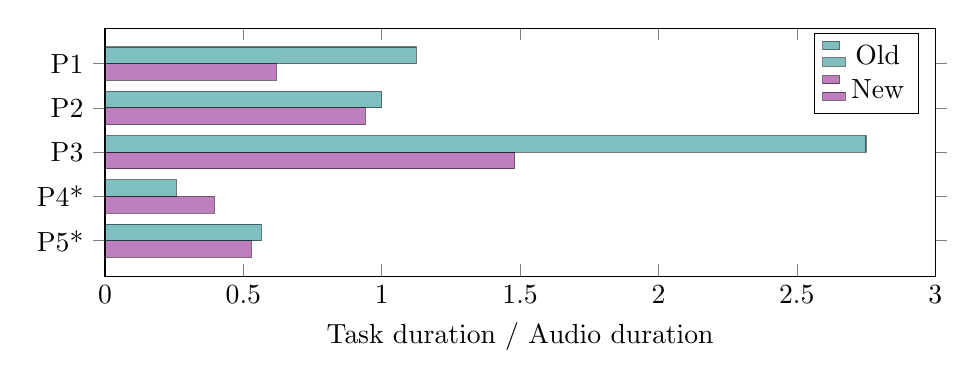
\begin{tikzpicture}
  \begin{axis}[
      width=\columnwidth,
      xbar=0pt,
      bar width=6pt,
      xlabel=Task duration / Audio duration,
      y=16pt,
      xmin=0,
      xmax=3,
      enlarge y limits=0.2,
      symbolic y coords={P1,P2,P3,P4*,P5*},
      ytick = data,
      y dir=reverse,
      reverse legend,
      ]
  \addplot[fill=violet, opacity=0.5] coordinates {(0.619,P1) (0.941,P2) (1.48,P3) (0.395,P4*) (0.529,P5*)};
  \addlegendentry{New}
  \addplot[fill=teal, opacity=0.5] coordinates {(1.125,P1) (1.0,P2) (2.75,P3) (0.258,P4*) (0.565,P5*)};
  \addlegendentry{Old}
  \end{axis}
  \end{tikzpicture}
  \caption{Time taken to complete the observed task for each workflow, compared
    to the original audio length. Lower is better. *P4 and P5 did not do any
    logging in the old workflow.}
  \label{fig:time}
\end{figure}

The time taken to complete the observed tasks was recorded (see
Figure~\ref{fig:time}). As different recordings of different lengths were used
for the old and new workflows, the times are reported relative to the length of
the audio. The speech-to-text processing time was not included in the
calculation as this is done in the background.

For P1 and P3, the new workflow was approximately twice as fast as the old one.
P2 completed the tasks at about the same speed, but was slowed down in the new
workflow by having to find each clip they highlighted on the printed
transcript.

P4 and P5 did not do any logging during observation of the old workflow,
so they completed the task much faster than the other participants who did.
Despite this, the time for the new workflow was comparable to the old.

\subsection{Cognitive load}


%\begin{table}
  %\centering
  %\begin{tabular}{ r | c c c c c | c }
    %& P1 & P2 & P3 & P4 & P5 & Mean \\
    %\hline
    %Mental demand   & -5  & -9  & -2  & 5   & 4 & -1.4 \\
    %Physical demand & 0   & 4   & 0   & 13  & 0 & 3.4 \\
    %Temporal demand & -1  & 4   & -5  & 4   & 1 & 0.6 \\
    %Performance     & -2  & 7   & 0   & 2   & 5 & 2.4 \\
    %Effort          & -1  & -7  & 7   & -4  & 2 & -0.6 \\
    %Frustration     & -12 & 1   & -3  & 2   & 5 & -1.4 \\
    %\hline
  %\end{tabular}
  %\caption{Difference in NASA-TLX results between the old and new workflows.
    %Negative results indicate that the new workflow is better.}
  %\label{tab:tlx}
%\end{table}

After completing both tasks in the observation, the participants were asked to
rate both the old and new workflows using the raw NASA-TLX metrics
\cite{Hart1988}.  The results are shown in Figure~\ref{fig:tlx}.

With only five participants, it is not possible to draw any conclusions about
cognitive load from these results.  They indicate that the new system requires
slightly less effort and mental demand, and is less frustrating. However it is
considered more physically demanding, temporally demanding and to perform
worse. To put these results in context, we must look at what the participants
said in the interviews.

\section{Interview discussions}
This section discusses the themes that emerged from an analysis of the
interviews (stage 4) and from the observation stage (stage 3). RQDA was used to
identify suitable quotes for each theme.

\begin{figure}
\centering
  \begin{tikzpicture}
  \begin{axis}[
      width=0.8\columnwidth,
      height=0.8\columnwidth,
      bar width=6pt,
      xbar=0pt,
      xlabel=Mean TLX value ($0-100$ scale),
      y=16pt,
      xmin=30,
      xmax=60,
      enlarge y limits=0.15,
      symbolic y coords={Frustration,Effort,Performance,Temporal demand,Physical demand,Mental demand},
      ytick=data,
      legend pos=east,
      legend style={at={(1,0.5)},anchor=east},
      reverse legend,
      ]
  \addplot[fill=violet, opacity=0.5] coordinates {(44.5,Frustration) (53,Effort) (41,Performance) (51.5,Temporal demand) (48,Physical demand) (51,Mental demand)};
  \addlegendentry{New}
  \addplot[fill=teal, opacity=0.5] coordinates {(48,Frustration) (54.5,Effort) (35,Performance) (50,Temporal demand) (39.5,Physical demand) (54.5,Mental demand)};
  \addlegendentry{Old}
  \end{axis}
  \end{tikzpicture}
  \caption{Mean NASA-TLX results for each system. Lower is better.}
  \label{fig:tlx}
\end{figure}

\vfill
\clearcolumn
\subsection{Logging}
Interviews recorded for speech radio often cover complex topics in fine
detail. Keeping track of all the points raised and forming a compelling
narrative from them is a challenge.

\textit{``All the interviews overlap with each other terribly, and have got
  similar themes.''} (P4)

The skill of the producer is to \textit{``separate the wheat from the chaff''}
(P1, P3, P4) and to find the clips which will make an interesting programme.

\textit{``That's the basis of my job - to find great stuff and put it together.
  It's not difficult putting it together, it's finding the great stuff and
  finding connections between it. Getting rid of the non-great stuff is
  challenging and time-consuming, and it requires mental processing.''} (P1)

Logging helps this process by allowing producers to see, on screen or on paper,
what was said in each interview and when, without having to listen to it. It
also helps them structure their thoughts, identify themes running through
discussions, and make links between different interviews. However, the sheer
quantity of recordings means this process adds significant overhead.

\textit{``you've got an average of 45 mins per interview and in a series of
  three programmes you've got seven per programme, that's a lot of work''} (P3)

Writing the logs takes a lot of concentration as the producer must comprehend
what is being said, work out how it ties in with other contributions and the
story, and make swift judgements on whether it should be used.

\textit{``one of the slightly exhausting things about doing it is the level of
  concentration you have to maintain to make good decisions, remember where
  everything is, what you've got, is kind of strained rather by having to just
  do shleppy tasks like moving the sound and logging interviews''} (P3)

Additionally, the open plan office in which producers work is not the best
environment for writing logs. For this reason, many choose to do it away from
the office. 

\textit{``I typically do this at home because I find it a much less distracting
  environment. It does require quite intensive concentration so you don't miss
  something.''} (P1)

The high level of concentration required, combined with the repetition of 
typing and listening to the interview again means that it is not enjoyable for
the producers.

\textit{``it's boring and it's not very easy to be efficient at it [...] when
  I'm normally doing it I'm checking my emails, making a cup of tea.''} (P3)

\subsection{Annotation}
The written logs created by the participants contained a number of annotations
to help them find important bits in the recordings later on. Each producer has
their own syntax, but there are common features.

Timestamps were written on the logs, approximately \textit{``every 30 to 120
  seconds''} (P1) with minutes and seconds in parenthesis: \texttt{(4'20)},
for example.  This allows the producer to navigate to a particular piece of
audio much faster than they would otherwise by narrowing down their search
range.

P1, P3 and P5 would make comments for themselves in the log to help them when
editing. For example, ``\textit{[good to here, dull after]}'' or
``\textit{[trails off 9'30]}''. P1 also used a star rating system to rate the
quality of each point, for example ``\textit{[**** should use this stuff, but
  dramatically cut down]}''.

\textit{``What I sometimes do when I edit are star good bits, and I think
  that's quite a common trait.''} (P3)

Bold highlighting was also used by P1 and P3 to mark bits of the transcript
which are important and worth keeping.

\textit{``what I did was just put in bold the paragraphs I thought were worth
  [keeping]''} (P1)

%In the observation stage, it was identified that annotation is an important
%part of the production process that was missing from the prototype.
When it came to using the semantic editing interface, there were no annotation
features available. This caused P1 and P3 to copy the transcript text from the
interface into Word so that they could make the desired annotations.

\textit{``it would be better to take raw lumps of transcripts and plonking them
  in Word because Word has higher functionality than this''} (P3)

Producers are very familiar with the Word interface so any new annotation
features should seek to match the user interface of such word processing
software.

\textit{``With text editing, the reflexes are very much Microsoft Word''} (P4)

The most basic feature that could be added is highlighting, which is often used
to note parts of interest

\textit{``If you just put a little star or underline or something simple to
  mark things, that would be a big gain for a small change''} (P3)

%\textit{``sufficient to find the bits of the audio you want to use and to make
  %sense to the presenter.''} (P3)

%\subsubsection{Star rating}

%\textit{`` I just gave myself a detailed breakdown of what was said in the
  %interview with timecodes at questions or major new points and a slightly
  %arbitrary scoring system to say 'that's really good stuff and must get in'.
  %''} (P1)

\subsection{Transcript navigation}
Participants suggested that having the transcript available in the semantic
editing interface allowed them to read and search the recordings much faster
than they normally would with a waveform.

\textit{``with having a transcript you're able to immediately scan through it
  10/15 times faster. Maybe that's an exaggeration but it feels ten times
  faster''} (P1)

Allowing users to click on a word to navigate to that point in the audio also
enabled them to use visual search to quickly find and listen to bits they were
looking for.

\textit{``you can do that with your eyes even quicker - zone straight in on the
  bits and that click to go  `that bit', `that sentence there', `that word
  there' ''} (P4)

%\subsubsection{Navigation speed}

%\textit{``it took me 15 mins to read 35 mins and not just read, but read and mark
  %up''} (P2)

%\subsubsection{Time since interview}

%\textit{``you're kind of doing a paper edit on the basis of having recently
  %heard the audio''} (P3)

%\textit{``a lot of that guesswork was coming from the memory of being there at
  %the recording... realising which bits were the questions from the
  %presenter and which bits were answers.''} (P2)

%\textit{``I know I've got a doc coming up in six months time, so I'll ask them
  %some questions for that. Now then in six months time I can't remember what
  %the answer was''} (P4)

%The primary benefit of reading over listening is that you can quickly scan
%ahead and jump around with your eyes, whereas listening can only be done at a
%fixed pace. 

In the old workflow, participants occasionally played the audio faster than
real time, but that feature was not included in the semantic editing system.
Several of the participants noted that they would like to have this
feature added.

\textit{``it's a little bit annoying that there's no facility for that.''}
(P2)

Although faster than real time playback normally reduces
intelligibility, this would be less of a problem if the transcript was
available \cite{Ranjan2006}.

\textit{``you do still need to listen through, even though you've got the text.
Therefore, it would be optimised if we could listen through quickly''}
(P4)

This would open the possibility for playback speeds faster than are currently
possible, allowing producers to listen to content much more quickly.

%Not all of the participants agreed though.
%\textit{``it wouldn't be something I'd be aching to be introduced''} (P1)

Although the Ctrl+F search feature that is included in web browsers is not a
designed feature of the semantic editor. It was discovered serendipitously and
was used to quickly find words in the transcript.

\textit{``it allowed me to get to clips very quickly from a reference point on
  a printed transcript''} (P2)

However P2 also noted that having timestamps on the printout would be a faster
way of achieving the same thing.

\subsection{Transcript accuracy}
Editing decisions must be made based on an automated transcript which is only
partially accurate. However, participants suggested that the transcripts were,
generally speaking, sufficiently accurate for their purposes, backing up 
previous research \cite{Whittaker2004}.

\textit{``It's clearly not 100\% in word recognition but I'm feeling it's
  certainly good enough for my rough cut purposes at this point''} (P2)

If the recording being edited was made recently, the producer can make up for
inaccuracies with the memory of what really happened.

\textit{``Both these interviews are relatively recent so I have it reasonably
  in my mind what they've been saying. I was able to read roughly what there
  was - `okay that's that question', `I know what was in that question' ''} (P1)

Although most producers only used the transcript to navigate and edit the
audio, some were interested in correcting the transcript so it could later be
shared or published.

\textit{``I'm probably posting transcripts for the whole interview. So I do
  need to go through and correct''} (P4)

The more accurate the transcript is, the less work has to be done to correct
it.

\textit{``The closer it can be to the point where you don't have to clean it up
  the better obviously, and that's quite significant honestly, that's my only
  qualm''} (P3)

%Sometimes a word is commonly mistranslated throughout the transcript, so
%providing an easy way to fix that would be a useful addition.

%\textit{``Something that would be even better is Ctrl+H  replace function''}
%(P3)

\subsection{Transcript editing}

Having the transcripts available allowed the participants to quickly cross
reference what was said in various interviews without having to listen through
multiple times.

\textit{``where I'm picking shorter clips, making a point and moving on or I'm
  developing an argument between different people and cutting between them, it
  feels a lot more easy to construct that on paper than what I'm currently
  doing''} (P2)

However it was also noted that the overhead of having wait for a transcript is
too much if the editing task is small.

\textit{``If it's a quick ten minutes with three questions, you don't need to
  bother''} (P3, also P4 and P5)

%\textit{``If it's a shorter thing I'll bang it straight into SADiE and start
  %editing down to find the wheat from the chaff''} (P4)

Editing with a transcript is primarily useful when working at the sentence
level. When the granularity of editing involves removing individual words,
`umm's or breaths, the DAW software is much better suited to these tasks. 

\textit{``the real editing work actually happens after this has passed its main
  point of usefulness''} (P3)

%\textit{``I was using some interviews, some contributors recorded on one
  %ocassion, but across several programmes, several episodes in a series, or for
  %several different stories.''} (P4)

%\subsection{Speaker diarization}
%One disadvantage of working with transcripts is that you can't hear which
%person is speaking when.

%\textit{``if you can't see who's speaking - that's a disadvantage''} (P3)

%Speaker diarization technology \cite{AngueraMiro2012} can be used to try and
%identify where different people are talking. The prototype included a
%rudimentary system that attempted to distinguish speakers and guess their
%gender, however it tended to significantly overestimate the number of speakers
%which caused some difficulty. 

%\textit{``It was distracting if anything, partly because I was trying to guess
  %who was which at certain points''} (P2)

%However, in many situations the participant could tell who was who from what
%they were saying.

%\textit{``It's reasonably clear to me who's asking the questions, but actually
  %[speaker diarization] is helpful''} (P1)

%During the study it was discovered that many producers record in stereo and use
%the waveform to see where people are speaking.

%\textit{``I always pan the presenter on one side and the contributor on the
  %other so I can see where the questions are''} (P5)

%This workaround could be exploited to improve the performance of a more
%advanced speaker diarization system.

\subsection{Interface design}
The semantic editing interface was designed so that the user could drag and
drop selected clips into an edit window. A major usability issue emerged when
the edit window filled up, as it was quite difficult to add clips to the end.

\textit{``I found the interface quite clunky for pulling out big chunks of
  audio.''} (P5)

Users worked around the problem by dropping new clips between old ones, then
re-ordering the new clip to the bottom of the list. One suggested fix was to
have a button to append a clip of the selected text to the edit without having
to drag and drop.

\textit{``once you've selected on the left hand side [...] it would go to the
  bottom of the queue, that would be a useful way of moving stuff from left to
  right for pulling highlight clips''} (P2)

Selecting very large amounts of text with a dragging motion also proved tricky,
so it was suggested that clicking whilst holding shift (like in word
processing) could fix this.

\textit{``Just being able to hold shift and use the cursor. Selecting the text
  was a little bit index finger intensive.''} (P4)

Although the semantic editor is set up to select good bits, a lot of the
participants also wanted to get rid of bad bits.

\textit{``What you need to do is [...] to get rid of the gubbins of me talking
  to presenters and mistranslating''} (P3)

Some were also interested in having cut functionality that would remove the
selected clip from the original recording. This would ensure that it can't be
used twice.

\textit{``You could even go further in the spirit of what it is which would
  being able to cut and paste, delete''} (P4)

%\subsubsection{Stage of usefulness}

%\textit{``The transcript is useful at a later stage in the production process
  %when I've cut my programmes, when I want to export clips to the news. When I
  %need to compile a final script for a presenter''} (P2)

\subsection{Paper}
In the observation stage, P2 chose to print out the transcript and work on
paper, which allowed them to work away from the screen.

\textit{``I'd prefer to do it on page than on screen. Just easier on my
  eyes.''} (P2)

Working on paper also allows producers to be productive outside of the office,
such as during their commute.

\textit{``What would be really useful would be to [...] take it away (say when
  I'm on the train going home) and I would paper edit the bits that I need''}
(P5)

%\textit{``In the office there's so much pressure and you're always doing stuff. When you
 %can step away from that, have a long commute, I can think''} (P5)

%Secondly, working on paper allows them to work anywhere, without requiring
%electricity.

%\textit{``It's highly portable. It doesn't require any power.''} (P2)

Another participant explained that for an upcoming programme, they were
planning to use a printed transcript to help them collaborate with their
presenter.

\textit{``we're just going to go through it with a pencil and paper, with a
  printout, and highlight the bits we want and cross out the bits we don't.''}
(P4)

%\subsection{TV}

%Two participants suggested that text-based editing would be equally, if not
%more, useful for TV production. P2, who formerly worked in television, said
%that their workflow already followed a similar pattern. 

%\textit{``If I was making a TV show this is what I would do. I'd effectively
  %print [a transcript], read, highlight, pull a collated collection of those
  %clips or number then, then write a draft script that combined everyone's
  %interview highlight clips that I thought were relevent for telling the
  %story.''} (P2)

%The costs involved in producting TV content are much higher than radio, so
%there is a greater financial incentive in streamlining the process.

%\textit{``There's an advantage to paper edit in TV because the assemblage
  %process takes longer and you might decide you don't need particular bits of
  %archive you thought you did and [save on] transfer costs.''} (P3)

\subsection{Listening}
Part of the appeal of having a transcript is that it frees the user from
listening to the audio in real-time. It also allows users to work on paper,
away from any electronic devices. However, disconnecting the audio from the
text fundamentally changes the production process.

\textit{``Radio is made with your ears. You'll never get away from that fact
  that you need to listen''} (P4, also P2, P3, P5)

The criteria for deciding whether a piece of audio is good enough to use in a
programme is not just about what was said, but how it was said. Making
decisions on whether to keep/lose something without listening to it isn't
desirable.

\textit{``How people say things is very important and I wouldn't want to lose
  that totally.''} (P5)

There was also concern that parts which sounded great but didn't come across
as well in the transcript may have been overlooked.

\textit{``I was anxious it might not have sounded as good as it read, or that I
  might be missing bits that sounded great ''} (P2)

As listening is an important part of the production process, text should remain
linked to the audio wherever possible to allow multi-modal interaction. Once
the link is broken, re-linking the two together can be costly.

%\subsubsection{Quantity}

%\textit{``We've got about six hours of audio for a one hour programme, and it's
  %all just one-on-one interviews''} (P4)

%\textit{``you've got to find the right bit which is burdonsome and annoying
  %when you've got 20 interviews to do''} (P1)

%\subsection{Export}

%Stuff on export and integration

%No gaps in WAV

\section{Follow-up}
After the interviews and observations were complete, the participants were given
access to the system for a further month (stage 5). During this time their
actions were logged electronically and they were asked each week about which
features they found useful, or were missing. P3 went on holiday immediately
after the study, so could not take part.

Most of the comments received in the follow-up stage were already picked up by
the first part of the study. In the remaining comments, all of the participants
said they enjoyed being able to use the semantic editor outside of the office
and at home, but had issues uploading content with their slow network
connections. P2 suggested that allowing multiple simultaneous uploads would
allow them to leave it running overnight.

\subsection{Usage}
The logs from the interface were analysed to see how the participants used the
system outside of the study, discover which features were being used, and for
how long.
All of the participants continued to use the semantic editor as part of their
work. The total time spent using the system in the follow-up period was 23
hours and 58 minutes.  Over 14 hours of those were from P2, with P4 using it
for 5 hours, P1 for 3 hours and P5 for 20 minutes.

\begin{figure}
\centering
  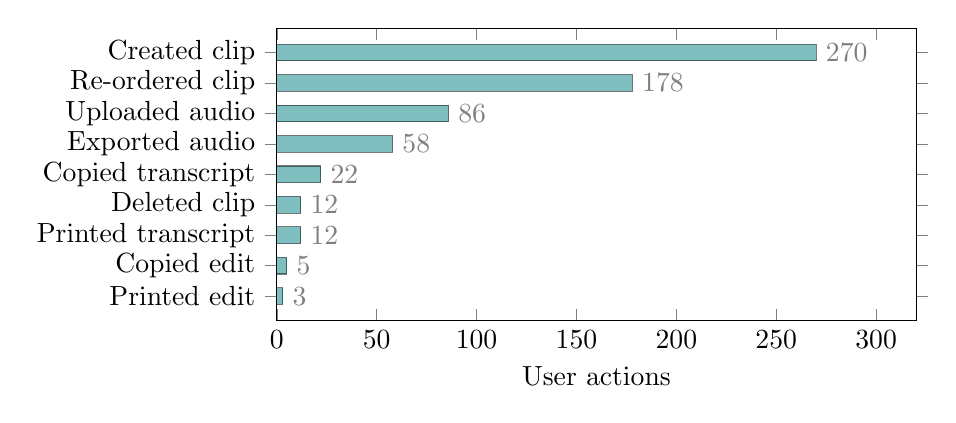
\begin{tikzpicture}
  \begin{axis}[
      width=0.8\columnwidth,
      %height=0.7\columnwidth,
      bar width=6pt,
      xbar=2pt,
      xlabel=User actions,
      y=11pt,
      xmin=0,
      xmax=320,
      symbolic y coords={Printed edit,Copied edit,Printed transcript,Deleted clip,Copied transcript,Exported audio,Uploaded audio,Re-ordered clip,Created clip},
      ytick=data,
      nodes near coords,
      ]
  \addplot[fill=teal, opacity=0.5] coordinates {(3,Printed edit) (5,Copied edit) (12,Printed
    transcript) (12,Deleted clip) (22,Copied transcript)
    (58,Exported audio) (86,Uploaded audio) (178,Re-ordered clip) (270,Created clip)};
  \end{axis}
  \end{tikzpicture}
  \caption{Count of logged user actions during follow-up}
  \label{fig:actions}
\end{figure}

Figure~\ref{fig:actions} shows that over 80 recordings were uploaded and over
50 audio edits were exported. The figure also shows that copying text was more
popular than printing. The large amount of re-ordering of clips is probably due
to the usability problem of running out of space in the edit window mentioned
in the `interface design' part of the interview discussion.

Users could navigate the content by either clicking on the waveform or by
clicking on a word in the transcript. In the interaction log, over 98\% of
navigation actions were executed by clicking on a word, which shows a clear
preference for navigating by text.

%\section{Implications}

%Remove as well as take away

%Annotation is import. Need to include word processing features

%Paper is still used, portable and easy on eyes

\section{Discussion}
%used a pilot study to identify an opportunity to use automatic transcripts of
%dialogue with synchronised audio to connect two previously separate activities
%in radio editing. This had mixed results as shown by the weak stats but more
%positive comments. It exposed some important missing functions like annotation
%and the importance of paper. The exercise also seems to have resulted n the
%first published study of documentary radio production.

% start with a summary and then extend each element at greater length

A pilot study of radio production identified an opportunity to make the
production of speech content more efficient by using automated transcripts to
enhance audio editing interfaces. In this study, we presented a semantic audio
editing system which allows users to navigate and edit speech using the
transcript text.  Previous studies \cite{Whittaker2004, Rubin2013} demonstrated
the potential of semantic editing, but this method had not been tested in a
professional production environment.

We conducted a qualitative study of five radio producers at the BBC to discover
how programmes are made, and to evaluate the semantic editing system. The study
found that current radio production practice involves spending a lot of time
creating logs of interviews,
%, which helps producers recall what was said and to
%structure and cross-reference material for their programmes.
which is lengthy, requires concentration and is considered
boring.

Our semantic editing system allowed the participants to log and edit long
recordings up to twice as fast as the existing technique, however the semantic
system was not as efficient for short recordings. The participants commented
that the semantic editing system allowed them to navigate and edit the audio
much faster, and that the accuracy of the transcript was good enough for their
purposes. Both of these results support previous findings
\cite{Whittaker2004,Rubin2013}.

Participants annotated their logs with timestamps and notes, and used star
ratings and highlighting to indicate important parts of their recordings. This
functionality was not included in the semantic editing system, which forced some
participants to import the text into Word to make annotations.
%This broke the connection between the audio and the text.
These annotation features could be added to the semantic editing system which
would allow the audio and transcript to remain linked.

The interface was designed so that users could select desired pieces of content
using a drag-and-drop technique. This design worked well for short clips, but
could not handle long clips. In addition to selecting content they did want,
participants were also interested in removing content that they didn't want. 
Enabling word processor style editing like cut, copy and paste would give the
users more freedom.
%TODO SO...

The participants often used paper to read and annotate their scripts and logs.
It is easier on their eyes, helps them to collaborate and allows them to be
productive away from the desk, such as during their commute.  During the study,
one participant went out of their way to edit on paper by printing and
highlighting the transcript.  Being able to move between the screen and paper
would bring the benefits of paper working and allow producers to use their time
more efficiently.

Finally, participants pointed out that ``radio is made with your ears''.
Editing decisions are based not only on what is said, but how it is said. This
emphasises the importance of a multi-modal interface, which combines the
efficiency of text-based working with being able to quickly listen back to the
audio.  Enhancing this with faster than real time listening would allow
users to review material at much faster speeds than they do already
\cite{Vemuri2004}.

In future work, we plan to improve the semantic editing interface by adding
faster than real time playback, and moving closer to a word processing style
design that includes cut, copy, paste, delete, undo and annotation features.
%We will also be investigating whether a
%similar system can be achieved on paper using digital pen technology.

%CONTIBUTIONS COMPARED TO OTHER WORK

%Logging helps producers to recall what was said in interviews and to structure
%and cross-reference

%Logging takes a long time, requires concentration and is boring.

%Producers annotate the logs with timestamps, notes, highlighting and star
%ratings.

%Word is used and preferred for making annotations

%Navigation using a transcript is considered faster

%There is a desire to listen to the audio faster than real time

%The transcript is accurate enough to do a rough edit

%A more accurate transcript would be beneficial

%The transcript interface is not needed for short recordings or fine editing

%Drag and drop clipping didn't work very well as it's hard to select long bits

%There is a desire for cut and delete functionality

%Working on paper is desirable

%Television could also benefit from this approach

%Need to listen to the audio

%Task completed up to twice as fast with the new system when including logging

%Participants continued to use the prototype after the study

%TODO
%move to a word like interface with cut, copy, paste, delete and annotation
%create a paper interface

%the paper needs some reflection on the aims and motivation at the end to
%underscore the lessons of the work and say what its contribution is compared
%with existing work

%\begin{itemize}
  %\item The process of logging and rough editing is an important part of radio
    %production, but is slow, boring and requires a high level of concentration.
  %\item Automated transcription is sufficiently good to replace the logging
    %process, but requires an easy way to make annotations.
  %\item Creating a rough edit using a transcript can be less mentally demanding
    %and up to twice as fast.
  %\item The participants voluntarily continued to use the prototype after the
    %study.
  %\item Listening is an important part of producing audio content.
%\end{itemize}

%Next
%\begin{itemize}
  %\item Develop and test method of link paper printouts to audio, perhaps using
    %digital pen technology
  %\item Conduct similar study for TV production
  %\item Develop method for keeping a script in-sync with the audio edit
%\end{itemize}

%%\textit{``There might be a version, a few steps down the track, where you cut
  %%the sound at the edit following along behind.''} (P3)

%A future version could try to
%emulate the word processing actions of highlighting and typing, or using
%context menus.

%The unexpected behaviour experienced in the observation suggests that the
%prototype is missing some desired features, namely the ability to make
%annotations, create a script and to integrate with paper.

%More advanced features could include a rating system for marking how important
%bits are on a scale.


